%% LaTeX template for the science justification & technical
%% feasibility to be submitted as part of a Chandra X-ray Observatory
%% proposal.
%%
%% Chandra Cycle 24


%%%%%%%%%%%%%%%%%%%%%%%%%%%
%%%%% DOCUMENT FORMAT %%%%%
%%%%%%%%%%%%%%%%%%%%%%%%%%%

%% The default font was chosen to be easily readable while allowing
%% sufficient material to be included.

%% The two-column, 11pt format fits the largest number of characters
%% per page while still being easily read.

%% There are three documentclass commands provided below. Please
%% uncomment the version you would like to use and comment out the
%% others.

%% Please note that the proposal requires US Letter size pages,
%% 8.5 in x 11 in. PLEASE DO NOT CHANGE THE 'LETTERPAPER' OPTION
%% IN THE DOCUMENTCLASS COMMAND.

\documentclass[letterpaper,11pt]{article}

%\documentclass[letterpaper,11pt,twocolumn]{article}

\renewcommand{\floatpagefraction}{.9}
\usepackage{graphics,graphicx}
\usepackage{sidecap}

% Numbered citations are standard in bibtex, but I also want to change
% the space between items i nthe biblography to save space.
% Only if I use natbib, I can do that by changing bibsep.
% So, use natbib and then switch that to numbers.
\usepackage[numbers,sort&compress]{natbib}
\setlength{\bibsep}{0pt plus 0.3ex}

%%%%%%%%%%%%%%%%%%%%%%%%%%%
%%%%% Page dimensions %%%%%
%%%%%%%%%%%%%%%%%%%%%%%%%%%

\setlength{\textwidth}{6.5in} 
\setlength{\textheight}{9in}
\setlength{\topmargin}{-0.0625in} 
\setlength{\oddsidemargin}{0in}
\setlength{\evensidemargin}{0in} 
\setlength{\headheight}{0in}
\setlength{\headsep}{0in} 
\setlength{\hoffset}{0in}
\setlength{\voffset}{0in}



%%%%%%%%%%%%%%%%%%%%%%%%%%%%%%%%%%
%%%%% Section heading format %%%%%
%%%%%%%%%%%%%%%%%%%%%%%%%%%%%%%%%%

\makeatletter
\renewcommand{\section}{\@startsection%
{section}{1}{0mm}{-\baselineskip}%
{0.5\baselineskip}{\normalfont\Large\bfseries}}%
\makeatother

\usepackage{xspace}

\newcommand{\sun}{$_{\odot}$\xspace}
\DeclareRobustCommand{\ion}[2]{%
\relax\ifmmode
\ifx\testbx\f@series
{\mathbf{#1\,\mathsc{#2}}}\else
{\mathrm{#1\,\mathsc{#2}}}\fi
\else\textup{#1\,{\mdseries\textsc{#2}}}%
\fi}

\def\farcm{\hbox{$.\mkern-4mu^\prime$}}
\def\farcs{\hbox{$.\!\!^{\prime\prime}$}}
\def\degr{\hbox{$^\circ$}}
\def\arcmin{\hbox{$^\prime$}}
\def\arcsec{\hbox{$^{\prime\prime}$}}

\def\aj{AJ}%

          % Astronomical Journal

\def\araa{ARA\&A}%

          % Annual Review of Astron and Astrophys

\def\apj{ApJ}%

          % Astrophysical Journal

\def\apjl{ApJ}%

          % Astrophysical Journal, Letters

\def\apjs{ApJS}%

          % Astrophysical Journal, Supplement

\def\ao{Appl.~Opt.}%

          % Applied Optics

\def\apss{Ap\&SS}%

          % Astrophysics and Space Science

\def\aap{A\&A}%

          % Astronomy and Astrophysics

\def\aapr{A\&A~Rev.}%

          % Astronomy and Astrophysics Reviews

\def\aaps{A\&AS}%

          % Astronomy and Astrophysics, Supplement

\def\azh{AZh}%

          % Astronomicheskii Zhurnal

\def\baas{BAAS}%

          % Bulletin of the AAS

\def\jrasc{JRASC}%

          % Journal of the RAS of Canada

\def\memras{MmRAS}%

          % Memoirs of the RAS

\def\mnras{MNRAS}%

          % Monthly Notices of the RAS

\def\pra{Phys.~Rev.~A}%

          % Physical Review A: General Physics

\def\prb{Phys.~Rev.~B}%

          % Physical Review B: Solid State

\def\prc{Phys.~Rev.~C}%

          % Physical Review C

\def\prd{Phys.~Rev.~D}%

          % Physical Review D

\def\pre{Phys.~Rev.~E}%

          % Physical Review E

\def\prl{Phys.~Rev.~Lett.}%

          % Physical Review Letters

\def\pasp{PASP}%

          % Publications of the ASP

\def\pasj{PASJ}%

          % Publications of the ASJ

\def\qjras{QJRAS}%

          % Quarterly Journal of the RAS

\def\skytel{S\&T}%

          % Sky and Telescope

\def\solphys{Sol.~Phys.}%

          % Solar Physics

\def\sovast{Soviet~Ast.}%

          % Soviet Astronomy

\def\ssr{Space~Sci.~Rev.}%

          % Space Science Reviews

\def\zap{ZAp}%

          % Zeitschrift fuer Astrophysik

\def\nat{Nature}%

          % Nature

\def\iaucirc{IAU~Circ.}%

          % IAU Cirulars

\def\aplett{Astrophys.~Lett.}%

          % Astrophysics Letters

\def\apspr{Astrophys.~Space~Phys.~Res.}%

          % Astrophysics Space Physics Research

\def\bain{Bull.~Astron.~Inst.~Netherlands}%

          % Bulletin Astronomical Institute of the Netherlands

\def\fcp{Fund.~Cosmic~Phys.}%

          % Fundamental Cosmic Physics

\def\gca{Geochim.~Cosmochim.~Acta}%

          % Geochimica Cosmochimica Acta

\def\grl{Geophys.~Res.~Lett.}%

          % Geophysics Research Letters

\def\jcp{J.~Chem.~Phys.}%

          % Journal of Chemical Physics

\def\jgr{J.~Geophys.~Res.}%

          % Journal of Geophysics Research

\def\jqsrt{J.~Quant.~Spec.~Radiat.~Transf.}%

          % Journal of Quantitiative Spectroscopy and Radiative Trasfer

\def\memsai{Mem.~Soc.~Astron.~Italiana}%

          % Mem. Societa Astronomica Italiana

\def\nphysa{Nucl.~Phys.~A}%

          % Nuclear Physics A

\def\physrep{Phys.~Rep.}%

          % Physics Reports

\def\physscr{Phys.~Scr}%

          % Physica Scripta

\def\planss{Planet.~Space~Sci.}%

          % Planetary Space Science

\def\procspie{Proc.~SPIE}%

          % Proceedings of the SPIE

\let\astap=\aap

\let\apjlett=\apjl

\let\apjsupp=\apjs

\let\applopt=\ao

%

\uchyph=0


%%%%%%%%%%%%%%%%%%%%%%%%%%%%%
%%%%% Start of document %%%%% 
%%%%%%%%%%%%%%%%%%%%%%%%%%%%%

\begin{document}
\pagestyle{plain}
\pagenumbering{arabic}


 
%%%%%%%%%%%%%%%%%%%%%%%%%%%%%
%%%%% Title of proposal %%%%% 
%%%%%%%%%%%%%%%%%%%%%%%%%%%%%

\begin{center} 
\bfseries\uppercase{%
%%
%% ENTER TITLE OF PROPOSAL BELOW THIS LINE
What happens after a stellar merger?
%%
%%
}
\end{center}

% This text is the abstract, but I'll show it again here because I don't want to rely on 
% people reading the separate forms.
One third of all stars are in binary or multiple systems \cite{Raghavan+2010}. If the components of a binary or multiple system are close enough to interact in some way, they can go through very different evolutionary pathways than single stars do. 
Many aspects of interacting binaries are subject to intense study, e.g.\ LIGO detections of neutron star or black hole mergers. However, stellar mergers can also happen in non-degenerate stars and this proposal requests observations to study one object that is strongly suspected to have undergone a recent merger: TYC 4144-329-2. 

Recent discovery of additional merger remnants and advanced modeling suggest the following sequence: As the primary expands, it causes its companion to spiral in and to transfer mass into a disk around the primary. As the companion is engulfed, the system launches outflows which are visible for a few thousand years. The merger remnant has a large radius, luminosity, and additional angular momentum compared to a giant that did not accrete a companion, all of which leads to the formation of a convective zone and an active dynamo, generating X-ray emission. As the star contracts, it spins up and its $L_\mathrm{X}/L_\mathrm{bol}$ increases while the outflow fades leading to FK Com systems. 

To test this hypothesis, we propose a 30~ks observation of TYC 4144-329-2, a suspected post-merger first-ascent giant branch star that is surrounded by an IR-bright disk. This system is later in the proposed sequence than BP Psc and  TYC 2597-735-1, two suspected merger remnants with outflows, but earlier than FK~Com which no longer has an IR disk. If the evolutionary sequence described above is correct, TYC 4144-329-2 should show more X-ray activity than BP Psc and  TYC 2597-735-1, but less than FK Com - a prediction easy to test with a Chandra observation.

 

\subsection*{The target TYC 4144-329-2}

\vskip -0.1in
Today, the target is a member of a wide ($> 5$ arcsec) binary. TYC 4144-329-2 itself is a F2-type first ascent giant star in a wide orbit with the otherwise normal  TYC 4144-329-1, a G8 IV \cite{2009ApJ...696.1964M}, but this system may have been a hirachical multiple in the past. Unlike other first-ascent giant stars, TYC 4144-329-2 is surrounded by a dust and gas disk that shows up as bright emission from the near-IR on (Fig~\ref{fig:SED}). Its spectral energy distribution (SED) mimics the SEDs of young stars with proto-planetary disks. 
%The disk around TYC 4144-329-2 has a luminosity close to one fifth of the stellar luminosity. A flat disk does not intercept enough stellar light to re-radiate that much emission, so the disk must be flared.
Black-body fits to the IR excess indicate a disk radius around 30~AU. The stellar spectrum of TYC 4144-329-2 shows emission lines which are associated with accretion in young stars, so it is likely that the inner edge of the disk is connected to the star and material falls in similar to the accretion streams in young T~Tauri stars \cite{2009ApJ...696.1964M}. 

TYC 4144-329-2's binary companion TYC 4144-329-1 can be used to age-date the system \cite{2009ApJ...696.1964M} to about 1 Gyr, far beyond the lifetime of proto-planetary disks of $<10$~Myr. The most plausible pathway to form such a disk in an evolved star is the consumption of a short-period companion, either a hot Jupiter or a low-mass stellar companion \cite{2009ApJ...696.1964M}. Depending on the orbital parameters and evolutionary pathway, the companion might have been destroyed in the process (\cite{2003ApJ...582.1032J}, compare also Fig.~\ref{fig:naturesketch} which describes a similar scenario) or could just be stripped of its outer atmosphere with a core that continues to orbit within the current gas and dust disk \cite{2003ASPC..293...76W}.


\begin{SCfigure}[][tb]
%\begin{center}
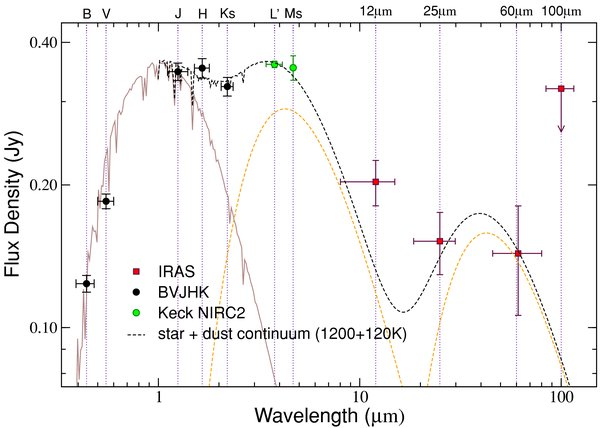
\includegraphics[angle=90,width=.5\textwidth]{SED}
\caption{Spectral energy distribution (SED) of TYC 4144-329-2 from \cite{2009ApJ...696.1964M}. The brown curve is a stellar model atmosphere, and the two yellow dashed lines show additional blackbody emission with 1200~K and 120~K temperature. The energy flux of those two additional components makes up about 17\% of the flux of the stellar model.}
\label{fig:SED}
%\end{center}
\end{SCfigure}


The accretion of a companion changes the properties of the atmosphere of the primary star. A lack of Li in TYC 4144-329-2 \cite{2009ApJ...696.1964M} indicates that the accreted object may itself not have been Li-rich, i.e.\ either it was massive enough to burn through its own Li in 1 Gyr (more massive than a brown dwarf) or it simply did not have enough mass to significantly pollute the phototosphere of TYC 4144-329-2 (e.g., a planet). More strikingly though, TYC 4144-329-2's optical lightcurve shows significant variability. It has been observed in three sectors by TESS and in all three epochs irregular variability $>10\%$ is seen. (Fig.~\ref{fig:TESS}). While TESS does not resolve TYC 4144-329-2 and TYC 4144-329-1, such variability is highly unusual for a normal subgiant and is thus likely associated with TYC 4144-329-2. The stellar merger process can lead to the formation of convective zones in the photosphere \cite{Soker&Tylenda2007} and a strong magnetic field \cite{Schneider+2016}, which power a convective dynamo and thus produce spots on the surface. While it is unlikely that this process alone is sufficient to explain the strong optical variability, \textit{a Chandra observation can test if magnetic coronal activity is present.}

\begin{SCfigure}
%\begin{center}
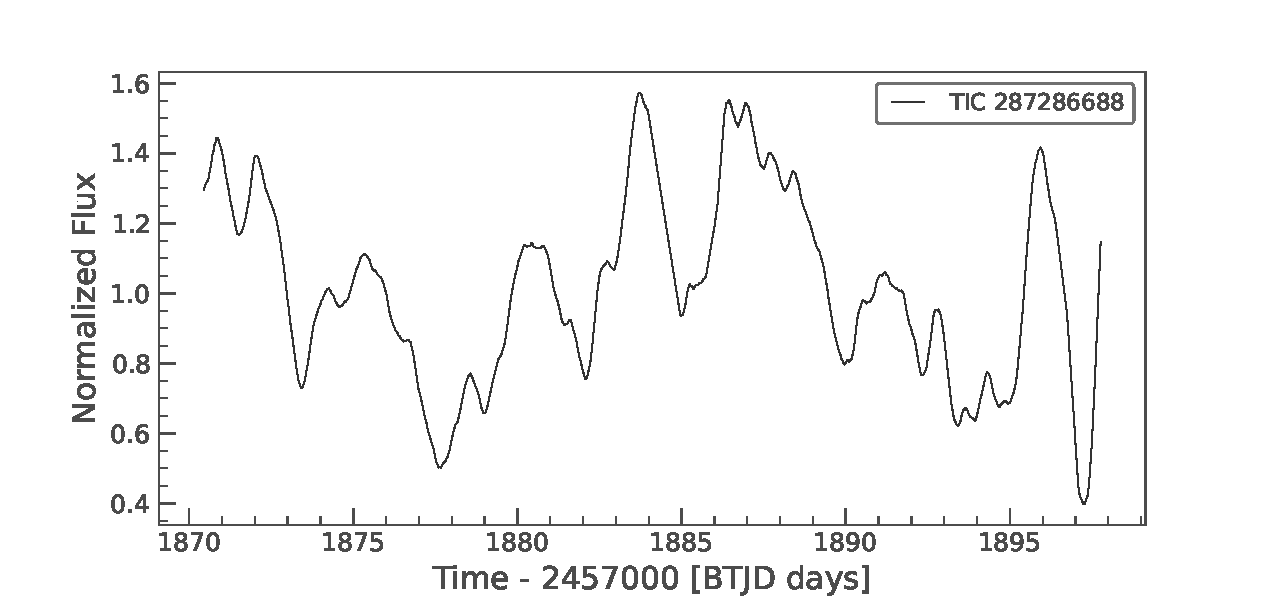
\includegraphics[angle=90,width=.5\textwidth]{TESSlc}
\caption{TESS Sector 21 Full Frame Image (30~minute cadence) lightcurve for TYC 4144-329-2 = TIC 287286688;
               flux is normalized to the maximum value seen in the plot. Significant variability is obvious, although no clear period is visible.}
\label{fig:TESS}
%\end{center}
\end{SCfigure}


\begin{figure}[htbp]
\begin{center}

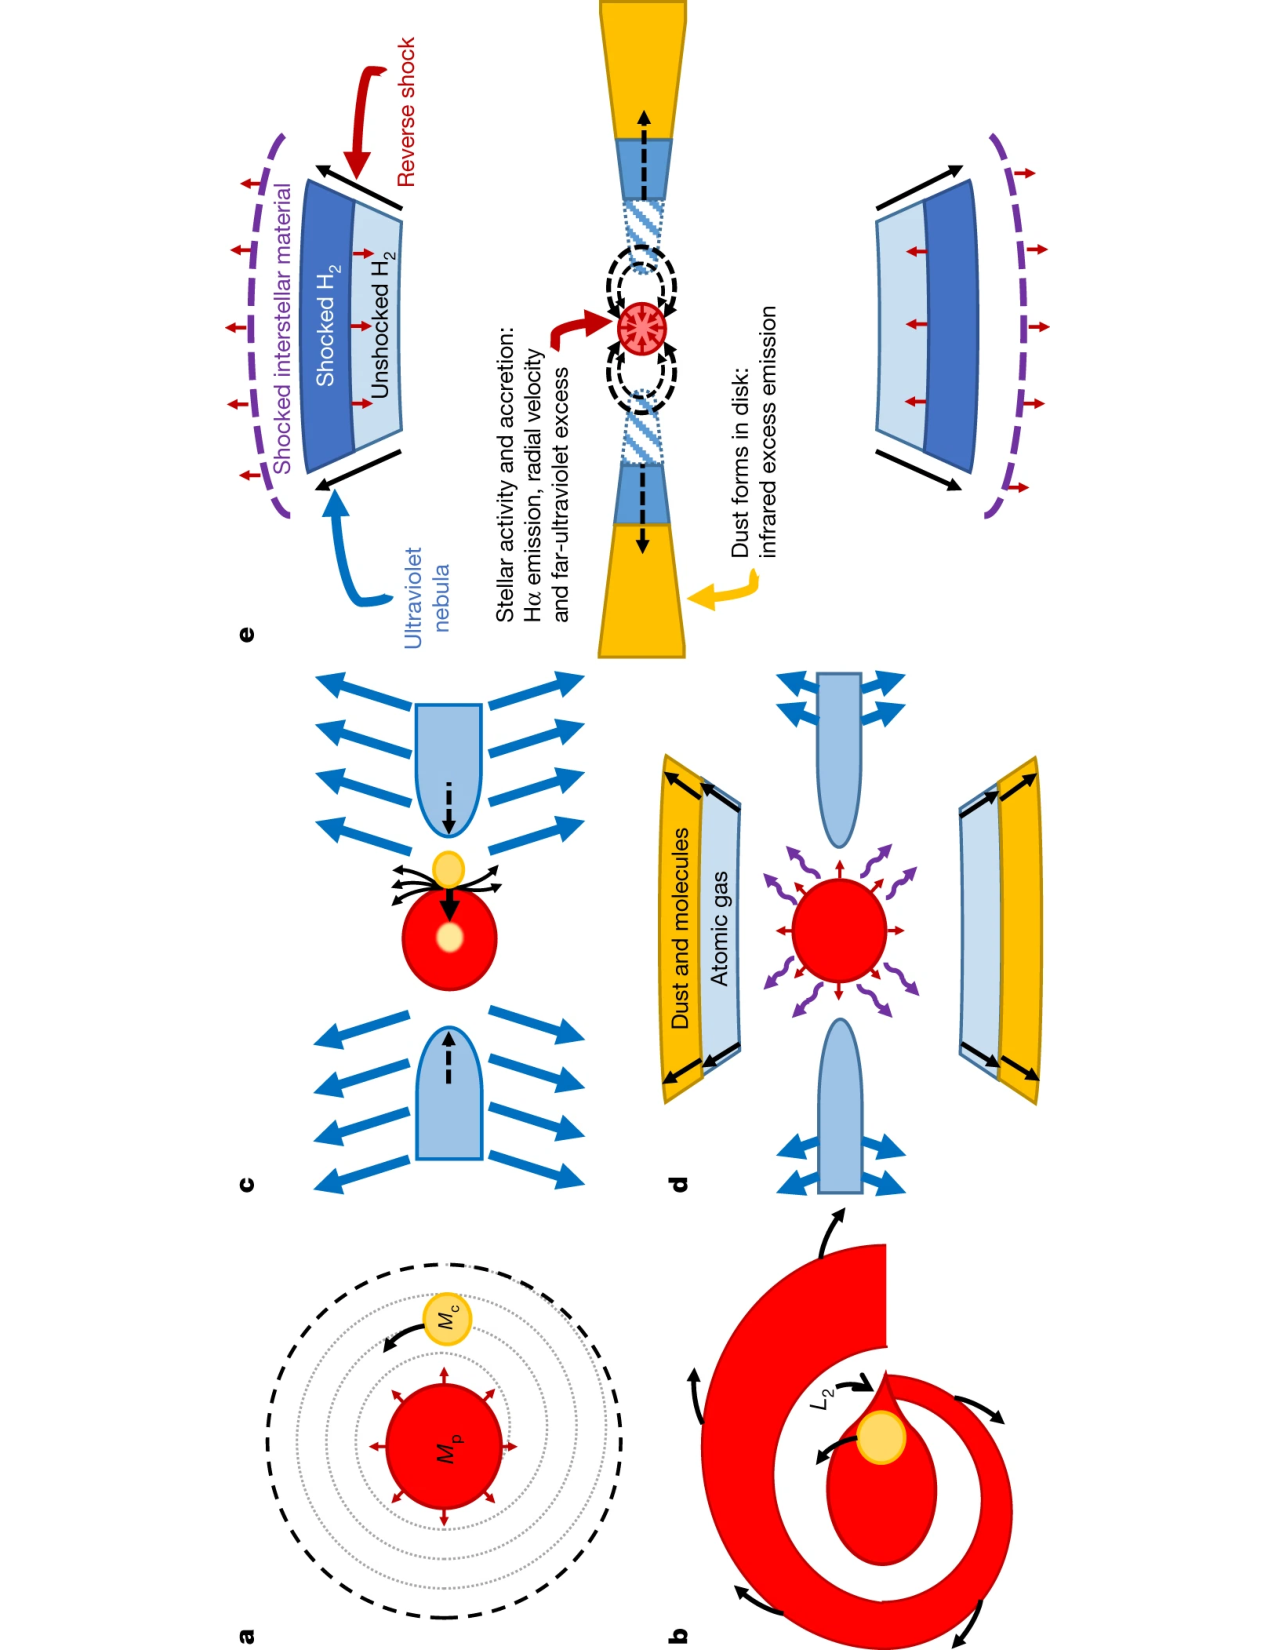
\includegraphics[angle=-90,width=.8\textwidth]{nature_sketch}
\caption{Possible pathway to form a disk by consuming a close companion as illustrated in \cite{2020Natur.587..387H}: As the primary star (red) evolves off the main-sequence, it expands, and drags in the companion (a, top view). The primary overflows its Roche lobe, but the companion cannot hold the mass, instead passing it through the Lagrange point L2 (b - top view). The companion falls into the primary, and the mass around L2 is shaped into a disk (c - side view). In TYC 2597-735-1 this leads to a bipolar outflow (d) which eventually shocks into the surrounding ISM (e).}
\label{fig:naturesketch}
\end{center}
\end{figure}





\subsection*{Science Objective: Tracing the evolutionary path from stellar merger to FK Com object}


\begin{SCfigure}
    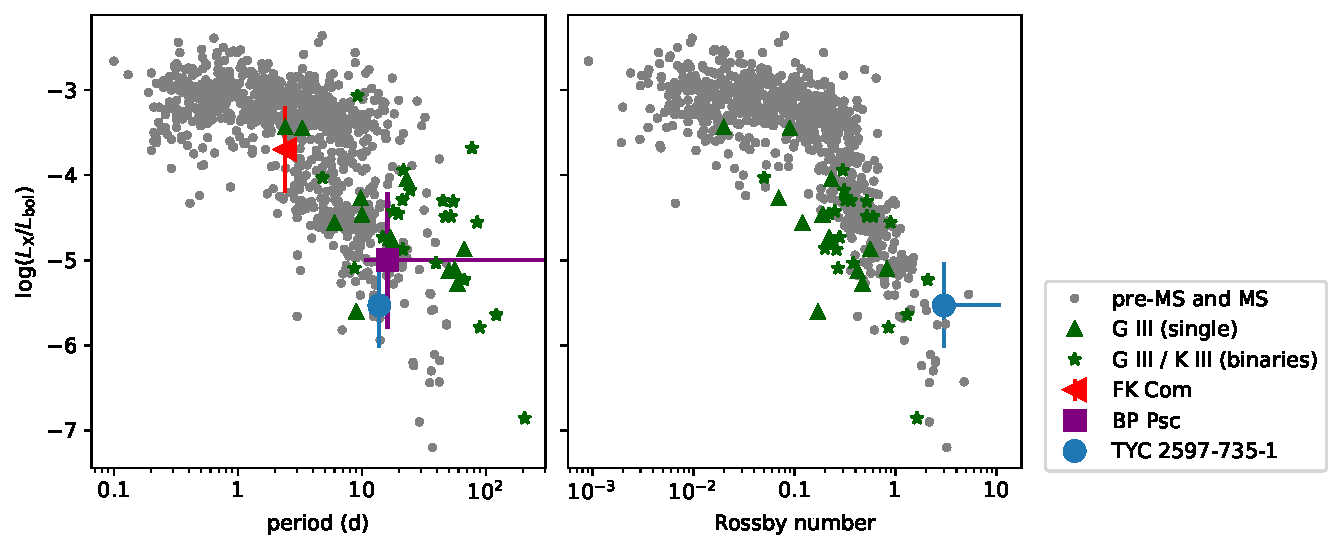
\includegraphics[width=.7\textwidth]{lxlbol}
    \caption{X-ray activity level for dwarfs and giants as a function of rotation period (left) and Rossby number (right). Suspected post-merger systems (blue, red, purple) follow the same trend as main-sequence stars and giants.  FK~Com is almost saturated, while BP Psc and TYC 2597-735-1 are significantly fainter (\cite{2022arXiv220205424G}).
    \label{fig:lxlbol}}
\end{SCfigure}

\vskip -0.1in
 TYC 4144-329-2 is among the  small group of suspected recent stellar merger remnants known today. Many of those stars are hidden behind significant gas and dust column densities, but 
 TYC 4144-329-2 is one of a few that can be seen in the optical \cite{2020RNAAS...4..238M} and potentially in X-rays. Other examples in this group are HD 233517 \cite{2003ApJ...582.1032J}, BP Psc \cite{Zuckerman_2008}, and  TYC 2597-735-1 \cite{2020Natur.587..387H}. Fig.~\ref{fig:naturesketch} shows the evolution of TYC 2597-735-1. As the primary star expands, it causes its companion to spiral in. After it engulfs the companion, it is surrounded by a dusty disk and also ejects a fast outflow. Similarly, BP~Psc shows an IR excess and also a light-year long highly collimated jet. Both these targets are detected in X-rays \cite{2010ApJ...719L..65K,2022arXiv220205424G}. Figure~\ref{fig:lxlbol} compares their $L_\mathrm{X}/L_\mathrm{bol}$ with main-sequence stars and single and binary giants. TYC 2597-735-1 and BP~Psc fall on the same $L_\mathrm{X}/L_\mathrm{bol}$-relation. As time goes on, their outflows will fade and the primary star will contract and spin up. When that happens, it seems plausible that these systems will develop into an FK~Com system - highly X-ray active giant stars \cite{2016ApJS..223....5A}, but without IR excess. How can this hypothesis be tested? This proposal requests observations of TYC 4144-329-2, a system with properties between 
TYC 2597-735-1 and BP~Psc on the one side and FK Com on the other side: TYC 4144-329-2 has no resolved outflow, but the IR disk is still around. \textbf{We propose a 30~ks of Chandra observation to test if TYC 4144-329-2 has an X-ray flux intermediate between TYC 2597-735-1 and BP~Psc  ($-5.5 < \log(L_\mathrm{X}/L_\mathrm{bol}) <-5$) and FK Com ($\log(L_\mathrm{X}/L_\mathrm{bol}) =-4$).}


\textit{Given the high incidence of binaries, understanding stellar binary mergers is important for a large number of stars and also limits the number of systems available for interaction in later stages (neutron stars, black holes).}

\subsection*{Feasibility}

\vskip -0.1in
The measured reddening for TYC 4144-329-2, $E_{B-V} = 0.32$, corresponds to $A_V = 1$ assuming interstellar-like grains \cite{2009ApJ...696.1964M}. This translates to $N_\mathrm{H} = 1.8\times10^{21}$~cm$^{-2}$ \cite{1995A&A...293..889P}. The bolometric luminosity of TYC 4144-329-2 is $16\;L_\odot$ and the distance 550~pc \cite{2009ApJ...696.1964M}.

While no rotational period has been directly observed, we can estimate a lower bound from the mass, surface gravity, and $v\sin i$ \cite{2009ApJ...696.1964M}. This gives a rotation period around 7 days assuming that we observe the equator. Looking at Figure~\ref{fig:lxlbol}, we can thus expect a $\log(L_\mathrm{X}/L_\mathrm{bol}) > -5.0$, the value seen for BP~Psc and possibly significantly higher. However, if the target turns out to be fainter, we want to be able to set an upper limit that proves it to be less X-ray active than BP~Psc and TYC~2597-735-1. Such an upper limit would rule out a shallow convective dynamo as proposed for TYC~2597-735-1 and reject the hypothesis that there is an evolutinary sequence from BP~Psc/TYC~2597-735-1 $\rightarrow$ our target $\rightarrow$ FK~Com. We thus design the observation to detect our target down to  $\log(L_\mathrm{X}/L_\mathrm{bol}) = -5.5$. According to WebPimms, the flux for ACIS-S is between 4 and 10 counts per 10~ks for plasma temperatures between 0.5 and 2 keV, typical for coronal plasma and consistent with the data from BP~Psc \cite{2010ApJ...719L..65K} and TYC 2597-735-1 \cite{2022arXiv220205424G}, which likely rotate slower. To safely detect the target even at this low flux, we request an exposure time of 30~ks. Given Poisson statistics, that gives us a $>99$\% chance of detecting the source with at least four photons even at the low end of the temperature range. We can apply a narrow band filter in just the 1-3~keV range, and thus background will be negligible. Only Chandra's PSF is good enough to safely distinguish TYC 4144-329-1 and TYC 4144-329-2 with a separation around 5 arcsec. This target has never been observed by pointed X-ray observations but was covered in the XMM slew survey a few times. The tightest limit is $6\times 10^{-13}$~erg/s/cm$^2$ in the 0.2-2.0~keV band, which corresponds to $\log L_\mathrm{X}/L_\mathrm{bol} < -3.8$. This limit is brighter than FK~Com and thus does not constrain our scenario.





%% Technical Justification for Joint Facilities section
%% comment this section out on proposals not asking for
%% joint time

%\section{Technical Justification for Joint Facilities}



%% References section

%\subsection*{References}


\bibliography{bib}{}
\bibliographystyle{plainetal}


%%%%%%%%%%%%%%%%%%%%%%%%%%%
%%%%% End of document %%%%%
%%%%%%%%%%%%%%%%%%%%%%%%%%%

\end{document}

